\section{Auswertung}
\label{sec:Auswertung}

\begin{figure}
  \centering
  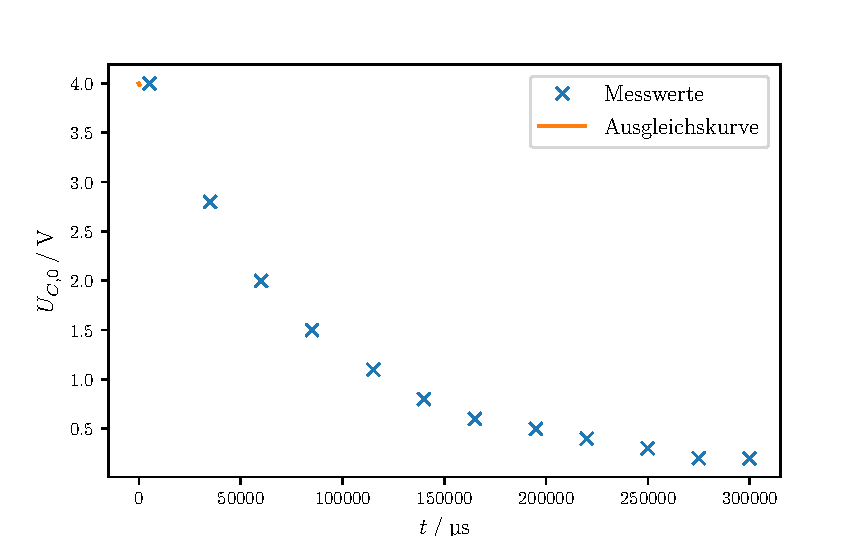
\includegraphics{build/plot1.pdf}
  \caption{Amplitudenmaximum der Kondensatorspannung eines RLC-Kreises in Abhängigkeit der Zeit.}
  \label{fig:plot}
\end{figure}
\begin{figure}
  \centering
  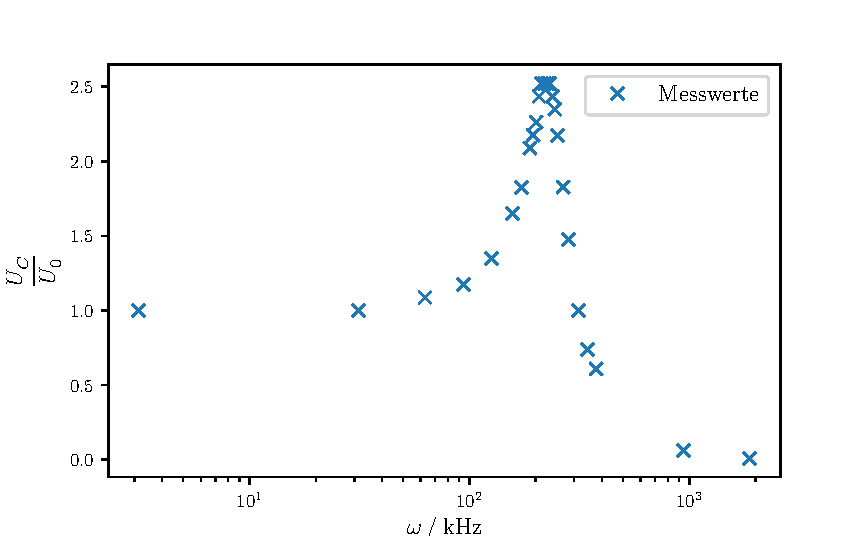
\includegraphics{build/plot2.pdf}
  \caption{Amplitudenmaximum der Kondensatorspannung eines RLC-Kreises in Abhängigkeit der Zeit.}
  \label{fig:plot}
\end{figure}

\begin{figure}
  \centering
  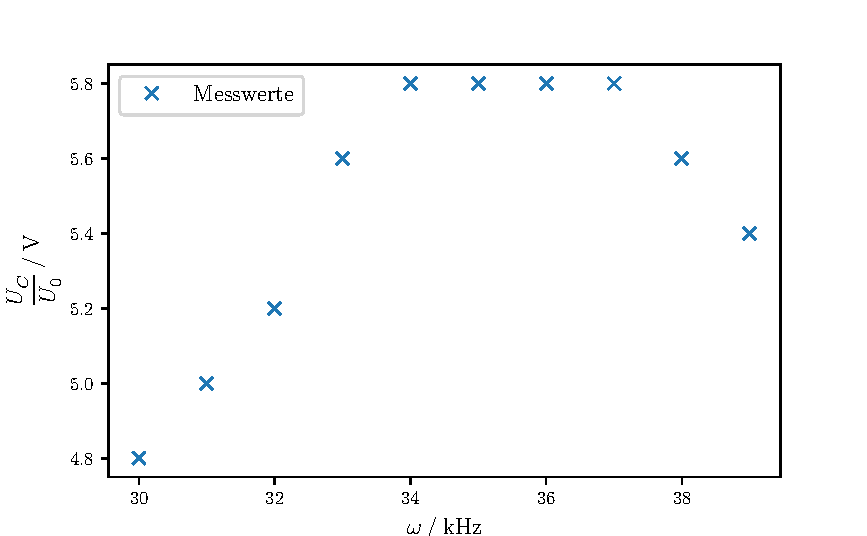
\includegraphics{build/plot3.pdf}
  \caption{Amplitudenmaximum der Kondensatorspannung eines RLC-Kreises in Abhängigkeit der Zeit.}
  \label{fig:plot}
\end{figure}






